% ----------------------------------------------------------------------
% Préambule
% ----------------------------------------------------------------------
\documentclass[12pt,a4paper]{article}
\usepackage[utf8]{inputenc}
\usepackage[T1]{fontenc}
\usepackage[french]{babel}
\usepackage{amsmath, amssymb, amsfonts}
\usepackage{booktabs}
\usepackage{graphicx}
\usepackage[hidelinks]{hyperref}
\usepackage[a4paper, inner=1cm, outer=1cm, top=2cm, bottom=2cm, bindingoffset=0cm]{geometry}
\usepackage{cmbright}
\setlength{\parindent}{0pt}

% Licence Creative Commons 4.0
\usepackage{ccicons}
\newcommand{\licence}{
\begin{center}
    \ccLogo\ \ccAttribution\ \ccShareAlike\ \ccVersionFour
    \\Ce document est sous licence Creative Commons CC BY-SA 4.0
\end{center}
}


\begin{document}

% ----------------------------------------------------------------------
% Page de couverture
% ----------------------------------------------------------------------
\begin{titlepage}
    \centering
    \vspace*{4cm}

    {\LARGE \textbf{Outils d'analyse d'un cours boursier}}\\[1.5cm]

    {\large $\ell$ouis tomczyk}\\[1cm]
    {\large \today}\\[2cm]

    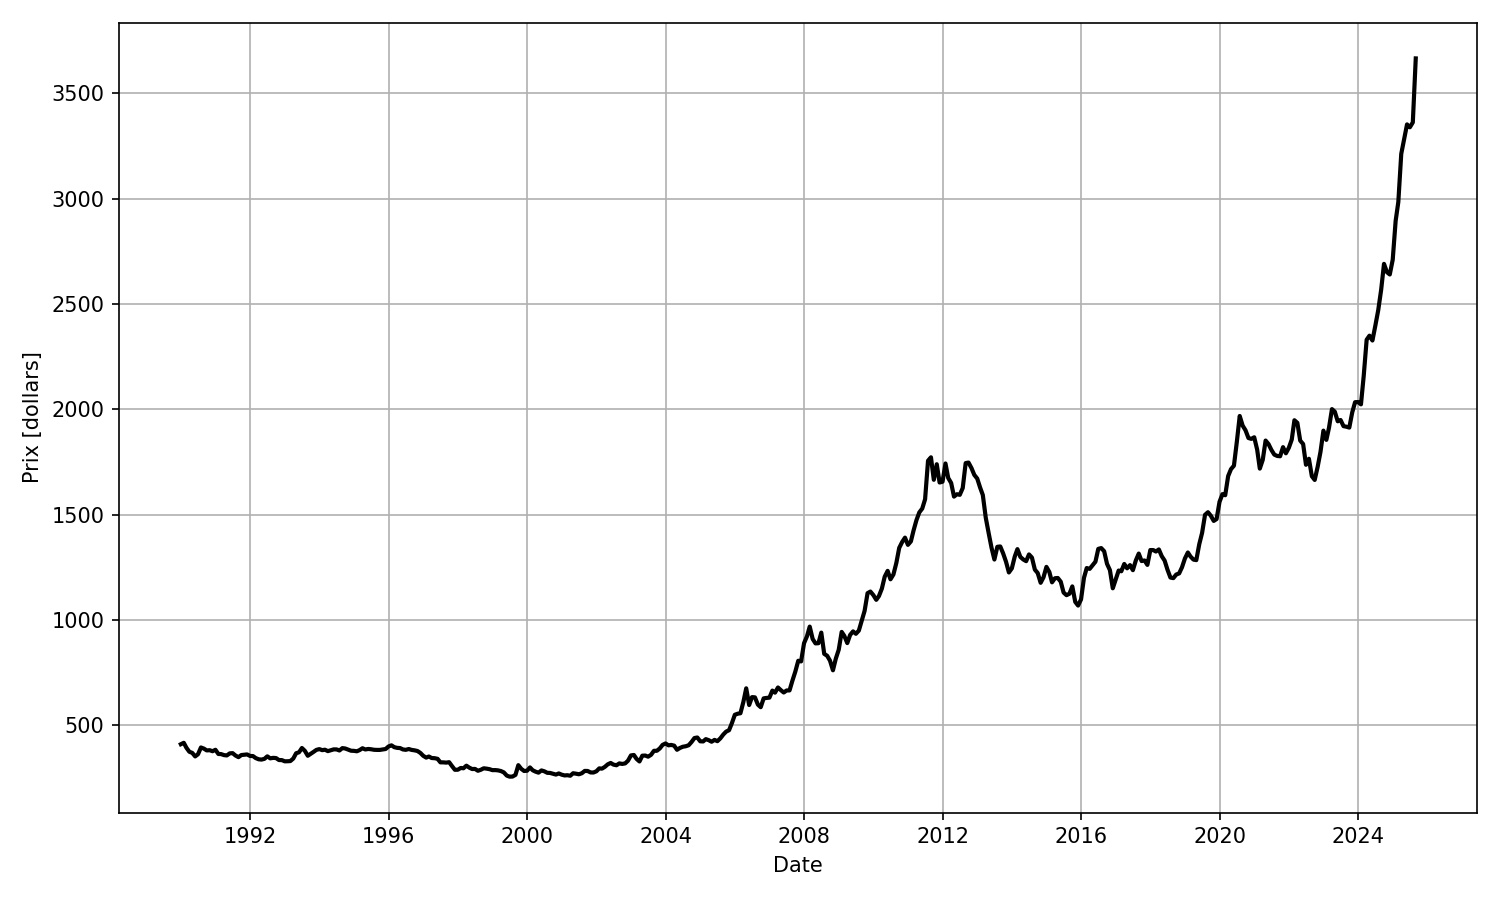
\includegraphics[width=\textwidth]{front.png}\\[2cm]

    % Licence Creative Commons
    \ccLogo\ \ccAttribution\ \ccShareAlike\\
    Ce document est publié sous licence Creative Commons CC BY-SA 4.0

    \vfill
\end{titlepage}

%\maketitle
\begin{abstract}
Ce document propose une introduction aux principaux outils financiers. Ces
outils sont calculés par un script Python pour analyser l'évolution des prix
mensuels de l'or. Destiné à un public scientifique, il vise à offrir une
présentation simplifiée des définitions, usages et interprétations, adaptée
à des lecteurs non spécialistes de la finance.
N'étant moi-même pas financier, ce document écrit avec une base fournie par
IA, est susceptible de contenir des erreurs et est nécessairement très
superficiel pour les professionnels du domaine. Enfin, ce document n'a pas
pour objectif de donner de conseils en investissements.
\end{abstract}

\tableofcontents
\newpage

%%%%%%%%%%%%%%%%%%%%%%%%%%%%%%%%%%%%%%%%%%%%%%%%%%%%%%%%%%%%%%%%%%%%%%%%%%%%%
%%%%%%%%%%%%%%%%%%%%%%%%%%%%%%%%%%%%%%%%%%%%%%%%%%%%%%%%%%%%%%%%%%%%%%%%%%%%%
%%%%%%%%%%%%%%%%%%%%%%%%%%%%%%%%%%%%%%%%%%%%%%%%%%%%%%%%%%%%%%%%%%%%%%%%%%%%%
\section{Données de base}

Les données sont mensuelles, au format CSV "date;prix" par exemple~:
\texttt{2025-09;3665.2}. Le prix est le cours spot (par once) et la
colonne \texttt{date} est convertie en index temporel (début du
mois, \texttt{MS}).
Ces données peuvent être obtenues sur le site de l'INSEE~:
{\scriptsize
\href{https://www.insee.fr/fr/statistiques/serie/010002061\#Telechargement}{https://www.insee.fr/fr/statistiques/serie/010002061\#Telechargement}}

%%%%%%%%%%%%%%%%%%%%%%%%%%%%%%%%%%%%%%%%%%%%%%%%%%%%%%%%%%%%%%%%%%%%%%%%%%%%%
%%%%%%%%%%%%%%%%%%%%%%%%%%%%%%%%%%%%%%%%%%%%%%%%%%%%%%%%%%%%%%%%%%%%%%%%%%%%%
%%%%%%%%%%%%%%%%%%%%%%%%%%%%%%%%%%%%%%%%%%%%%%%%%%%%%%%%%%%%%%%%%%%%%%%%%%%%%
\section{Rendements}

%%%%%%%%%%%%%%%%%%%%%%%%%%%%%%%%%%%%%%%%%%%%%%%%%%%%%%%%%%%%%%%%%%%%%%%%%%%%%
\subsection{RS~: Rendement simple}
Le rendement simple entre deux mois consécutifs est défini par~:
$
\boxed{RS = \frac{P_t - P_{t-1}}{P_{t-1}}}.
$
C'est la variation relative du prix d'un mois à l'autre. Il est
sans dimension (par exemple, 0.05 = +5\%). Ce nombre est immédiat
mais non-additif dans le temps, ce qui complique son agrégation.

%%%%%%%%%%%%%%%%%%%%%%%%%%%%%%%%%%%%%%%%%%%%%%%%%%%%%%%%%%%%%%%%%%%%%%%%%%%%%
\subsection{RLog~: Rendement logarithmique}
On définit le rendement logarithmique par~:
$
\boxed{RLog = \ln\left(P_t/P_{t-1}\right)}
$
Il est approximativement égal au rendement simple pour de petites
variations et a l'avantage d'être additif~: la somme des rendements
logarithmiques est le rendement logarithmique cumulé. Ceci en fait
un choix naturel pour l'analyse stochastique et la modélisation.

%%%%%%%%%%%%%%%%%%%%%%%%%%%%%%%%%%%%%%%%%%%%%%%%%%%%%%%%%%%%%%%%%%%%%%%%%%%%%
\subsection{RA~: Rendement moyen annualisé}
Si les rendements mensuels sont constants à
\(r_{m}\), alors le rendement annuel est~:
$
\boxed{R_{ann} \approx (1+\bar r_{m})^{12} - 1}.
$
Cette transformation permet de comparer la performance moyenne annuelle (le 12)
aux autres actifs ou indices, mais n'est pas adapté si les rendements évoluent.
On lui préfère le CAGR définit plus après.

%%%%%%%%%%%%%%%%%%%%%%%%%%%%%%%%%%%%%%%%%%%%%%%%%%%%%%%%%%%%%%%%%%%%%%%%%%%%%
%%%%%%%%%%%%%%%%%%%%%%%%%%%%%%%%%%%%%%%%%%%%%%%%%%%%%%%%%%%%%%%%%%%%%%%%%%%%%
%%%%%%%%%%%%%%%%%%%%%%%%%%%%%%%%%%%%%%%%%%%%%%%%%%%%%%%%%%%%%%%%%%%%%%%%%%%%%
\section{Moyennes mobiles}

%%%%%%%%%%%%%%%%%%%%%%%%%%%%%%%%%%%%%%%%%%%%%%%%%%%%%%%%%%%%%%%%%%%%%%%%%%%%%
\subsection{SMA~: Simple Moving Average}
La SMA sur \(n\) périodes est~:
\begin{equation}
SMA_n(t) = \frac{1}{n} \sum_{k=0}^{n-1} P_{t-k}.
\end{equation}
Elle lisse les oscillations à court terme~; si le prix est au-dessus
de la SMA, cela signale une tendance haussière relative sur la fenêtre
considérée.

%%%%%%%%%%%%%%%%%%%%%%%%%%%%%%%%%%%%%%%%%%%%%%%%%%%%%%%%%%%%%%%%%%%%%%%%%%%%%
\subsection{EMA~: Exponential Moving Average}
L'EMA (Exponential Moving Average) est une moyenne mobile pondérée
de manière exponentielle, définie par la relation récursive~:

\begin{equation}
    EMA_t = \alpha P_t + (1-\alpha) EMA_{t-1}, \quad
    \alpha = \frac{2}{n+1},
\end{equation}

où $P_t$ est le prix à l'instant $t$, $n$ la durée de l'EMA, et $\alpha$ 
le facteur de lissage.

\newpage
\textbf{Interprétation~:}
\begin{itemize}
  \item L'EMA donne un poids plus important aux valeurs récentes,
        contrairement à la SMA (Simple Moving Average) qui pèse chaque
        valeur de manière égale.
  \item Elle réagit donc plus rapidement aux changements de tendance,
 ce qui est utile pour détecter des inflexions ou des accélérations de prix.
  \item La constante $\alpha$ contrôle la réactivité~: plus $n$ est petit,
        plus $\alpha$ est grand et l'EMA suit de près le prix actuel.
\end{itemize}

\textbf{Momentum~:}  
Le \emph{momentum} mesure la variation des prix sur une période donnée~:
$M_t = P_t - P_{t-k}$ où $k$ est le nombre de périodes considérées.  
Un momentum positif indique une tendance haussière, tandis qu'un momentum négatif 
indique une tendance baissière. L'EMA permet de filtrer le bruit pour mieux 
visualiser le momentum sous-jacent.

\textbf{Exemples d'usage~:}
\begin{itemize}
  \item EMA courte (ex.~12 mois) pour détecter des signaux rapides,
        EMA longue (ex.~26 mois) pour filtrer le bruit.
  \item Les croisements EMA courte / EMA longue servent de signaux
        d'achat ou de vente.
\end{itemize}

\textbf{Remarque~:}  
L'EMA peut être vue comme une somme pondérée des prix passés avec un 
poids décroissant exponentiellement, analogue à un filtre passe-bas 
en physique du signal.

%%%%%%%%%%%%%%%%%%%%%%%%%%%%%%%%%%%%%%%%%%%%%%%%%%%%%%%%%%%%%%%%%%%%%%%%%%%%%
\subsection{Bandes de Bollinger}
On définit la bande centrale comme la SMA sur 20 périodes
et les bornes comme $\pm 2$ fois l'écart-type mobile~:
\begin{eqnarray}
    BB_{mid} = SMA_{20}(P_t), &\quad
    BB_{sup} = BB_{mid} + 2\sigma_t, &\quad
    BB_{inf} = BB_{mid} - 2\sigma_t.
\end{eqnarray}

L'écartement des bandes mesure la volatilité locale~; un prix qui
s'écarte fortement des bandes peut indiquer une condition extrême.

\begin{figure}[ht]
    \centering
    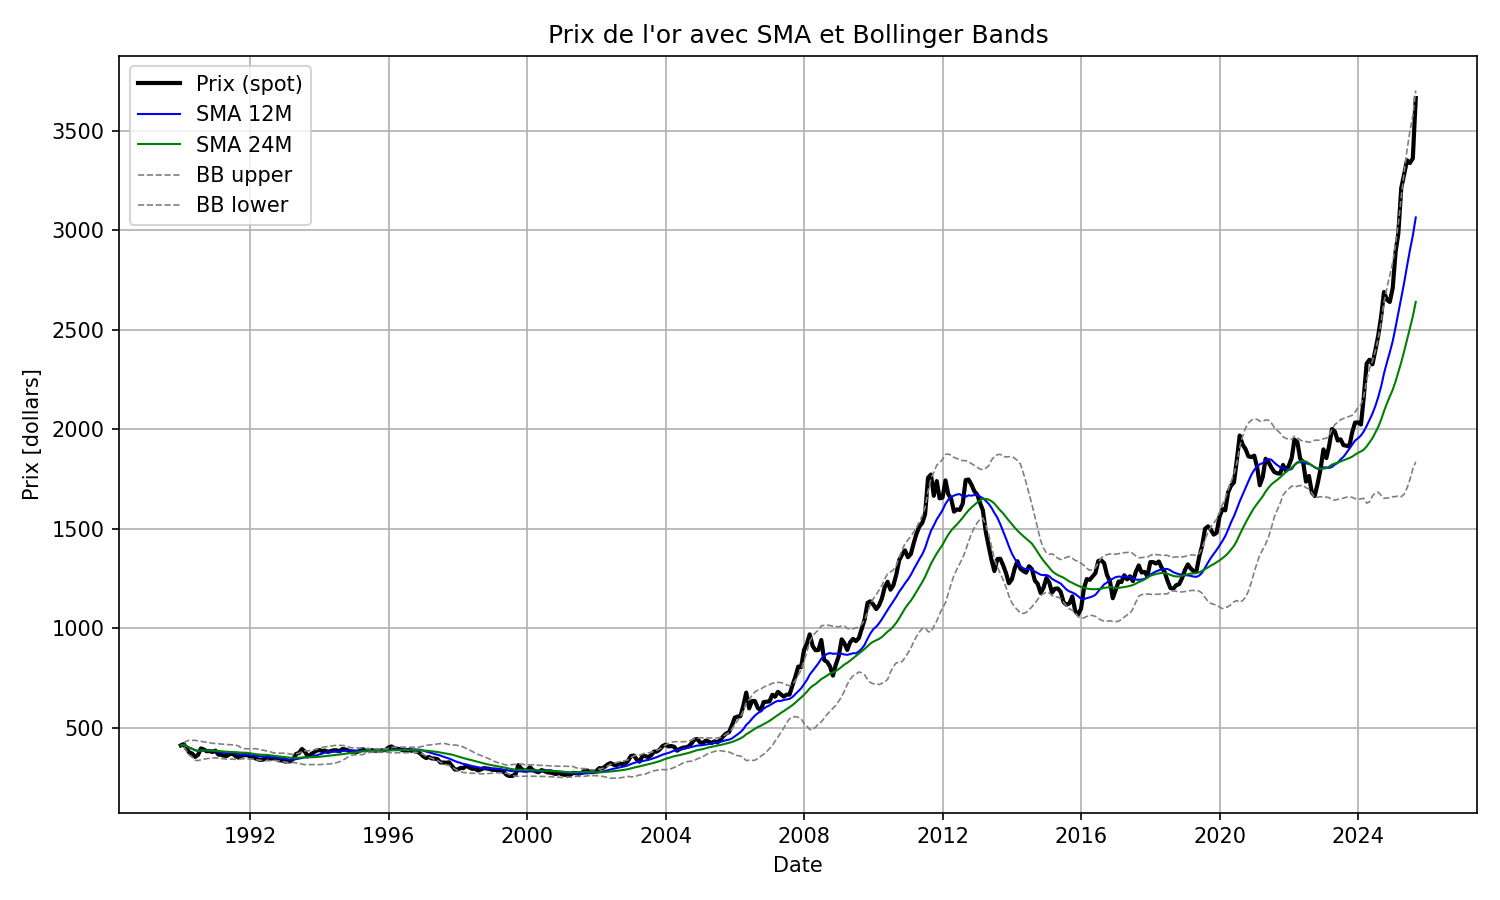
\includegraphics[width = 0.9\textwidth]{gold_price_sma_bb.png}
    \caption{Illustration de moyennes mobiles sur le cours de l'or avec 
                les Bollinger bands.}
    \label{fig:gold_price_sma_bb}
\end{figure}


%%%%%%%%%%%%%%%%%%%%%%%%%%%%%%%%%%%%%%%%%%%%%%%%%%%%%%%%%%%%%%%%%%%%%%%%%%%%%
%%%%%%%%%%%%%%%%%%%%%%%%%%%%%%%%%%%%%%%%%%%%%%%%%%%%%%%%%%%%%%%%%%%%%%%%%%%%%
%%%%%%%%%%%%%%%%%%%%%%%%%%%%%%%%%%%%%%%%%%%%%%%%%%%%%%%%%%%%%%%%%%%%%%%%%%%%%
\newpage
\section{Indicateurs de momentum}

%%%%%%%%%%%%%%%%%%%%%%%%%%%%%%%%%%%%%%%%%%%%%%%%%%%%%%%%%%%%%%%%%%%%%%%%%%%%%
\subsection{MACD~: Moving Average Convergence Divergence}

Le MACD (Moving Average Convergence Divergence) est un indicateur de momentum 
calculé à partir des différences entre des moyennes mobiles exponentielles (EMA) de 
durées différentes~:
\begin{eqnarray}
    MACD    = EMA_{12} - EMA_{26}, &\quad
    Signal  = EMA_9(MACD), &\quad
    Hist    = MACD - Signal.
\end{eqnarray}

\paragraph{Interprétation~:}
\begin{itemize}
    \item \textbf{MACD~:} mesure la différence entre EMA rapide et EMA lente. 
          Positive si le prix récent croît plus vite que la moyenne historique ;
          négative si le prix ralentit.
    \item \textbf{Signal~:} lissage du MACD sur 9 périodes. Sert de ligne de 
          référence pour identifier les changements de momentum.
    \item \textbf{Hist~:} histogramme représentant l'écart entre la MACD et le Signal. 
          Il visualise la vitesse de variation du MACD~: 
          \begin{itemize}
              \item Hist positif et croissant~: accélération haussière,
              \item Hist négatif et décroissant~: accélération baissière.
          \end{itemize}
\end{itemize}

\paragraph{Exemples numériques typiques~:}
\begin{itemize}
    \item MACD~: $-1$ à $+2$ en $USD$ pour l'or sur données mensuelles,
    \item Signal~: suit le MACD mais plus lissé, valeurs proches de $-0.8$ à $+1.8$,
    \item Hist~: petits écarts typiques $-0.5$ à $+0.5$ USD, 
          permet de détecter des retournements rapides.
\end{itemize}

\paragraph{Usage pratique~:}
\begin{itemize}
    \item Croisement du MACD au-dessus de Signal~: momentum haussier, possible début 
          de tendance.
    \item Croisement du MACD au-dessous de Signal~: momentum baissier, possible 
          correction.
\end{itemize}

\begin{figure}[ht]
    \centering
    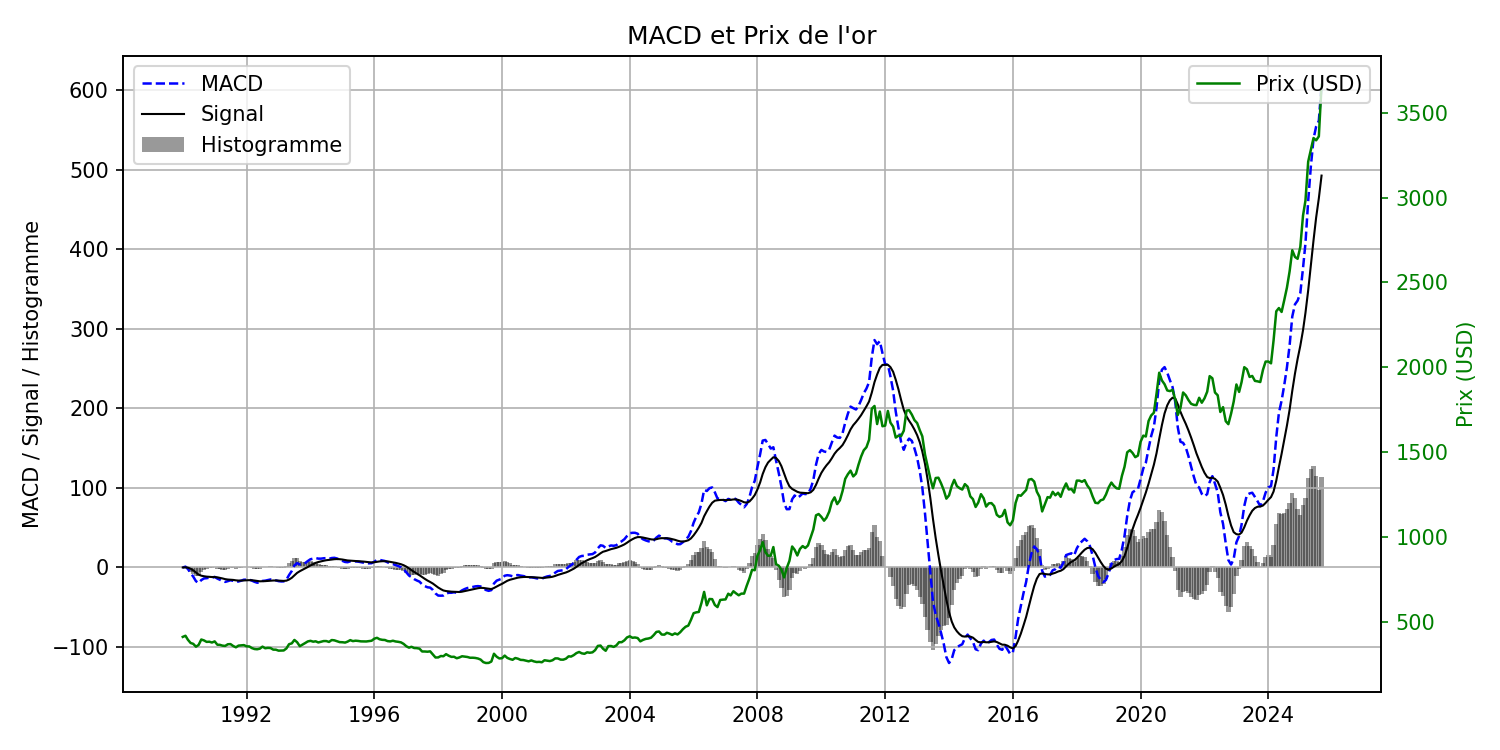
\includegraphics[width = 0.9\textwidth]{gold_macd_doubly_axis_colored.png}
    \caption{Illustration du MACD sur le cours de l'or avec sa vitesse de variation.}
    \label{fig:gold_macd_doubly_axis_colored}
\end{figure}


%%%%%%%%%%%%%%%%%%%%%%%%%%%%%%%%%%%%%%%%%%%%%%%%%%%%%%%%%%%%%%%%%%%%%%%%%%%%%
\newpage
\subsection{RSI~: Relative Strength Index}
Le RSI normalisé sur une période $N$ (classiquement $N=14$) est~:
\begin{equation}
    RSI = 100 - \frac{100}{1 + RS},\quad RS = \frac{\text{gain moyen}}{\text{perte
moyenne}}.
\end{equation}

Le RSI est un oscillateur borné entre 0 et 100~: typiquement
$RSI>70$ signale un \textit{surachat} et $RSI<30$ une \textit{survente}.
Ces seuils sont empiriques et peuvent varier selon les actifs. Pour l'or, des
tests statistiques (e.g., p-value du test ADF) pourraient valider leur pertinence
sur des données historiques.

\begin{figure}[ht]
    \centering
    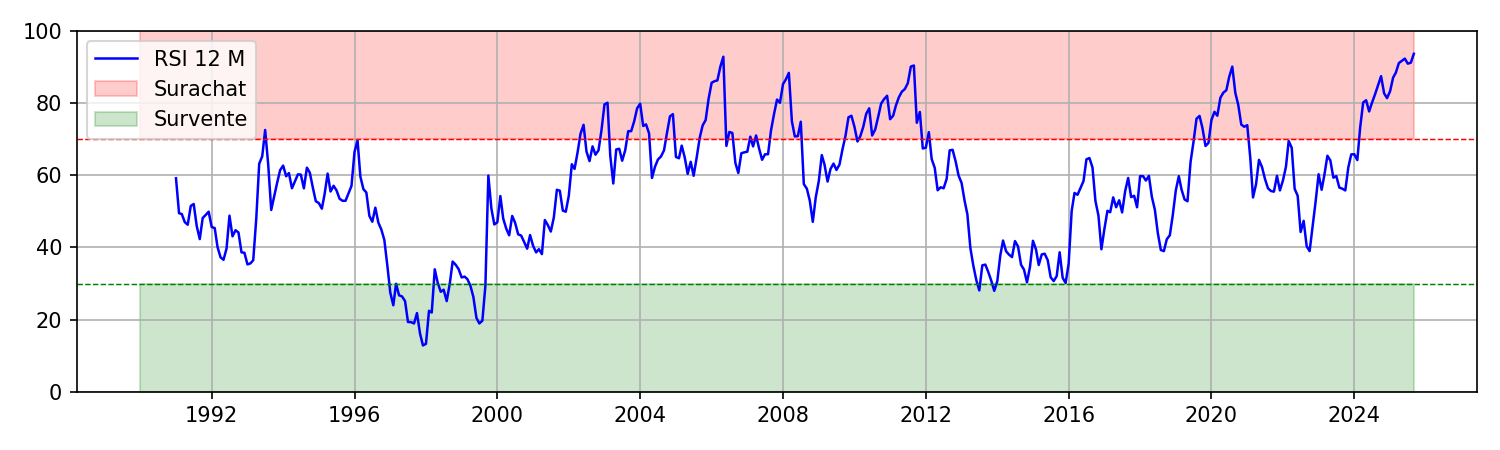
\includegraphics[width = 0.9\textwidth]{gold_rsi_zones.png}
    \caption{Illustration du MACD sur le cours de l'or avec sa vitesse de variation.}
    \label{fig:gold_rsi_zones}
\end{figure}



%%%%%%%%%%%%%%%%%%%%%%%%%%%%%%%%%%%%%%%%%%%%%%%%%%%%%%%%%%%%%%%%%%%%%%%%%%%%%
%%%%%%%%%%%%%%%%%%%%%%%%%%%%%%%%%%%%%%%%%%%%%%%%%%%%%%%%%%%%%%%%%%%%%%%%%%%%%
%%%%%%%%%%%%%%%%%%%%%%%%%%%%%%%%%%%%%%%%%%%%%%%%%%%%%%%%%%%%%%%%%%%%%%%%%%%%%
\section{Volatilité roulante}

La \textbf{volatilité roulante} mesure la variation du prix d'un actif sur une 
fenêtre glissante dans le temps. Elle est calculée comme l'écart-type des 
rendements logarithmiques sur une période donnée (ex. 12 mois pour des données 
mensuelles), puis annualisée pour être comparable à d'autres indicateurs financiers~:
\begin{equation}
    \sigma_{ann}(t) = \sqrt{12}\; \mathrm{std} \bigl(RLog_{t-11:t}\bigr),
\end{equation}
où $r_{t-11:t}^{(\ln)}$ représente la série des rendements logarithmiques des 12 
derniers mois.

\paragraph{Interprétation~:}
\begin{itemize}
    \item La volatilité indique l'amplitude typique des variations de prix~: 
          plus elle est élevée, plus le prix est instable.
    \item Une volatilité basse (inférieure au premier quartile historique) 
          correspond à un régime calme.
    \item Une volatilité élevée (supérieure au troisième quartile historique) 
          correspond à un régime turbulent ou incertain.
    \item Les pics de volatilité coïncident souvent un peu après les crises financières 
          ou géopolitiques (ex. 2008, 2020, 2022).  
          En effet~:
          \begin{enumerate}
              \item Lorsqu'une crise éclate, les prix commencent à chuter ou à bondir.
              \item Sur la fenêtre roulante (12 mois dans notre exemple), les variations
                    mensuelles s'ajoutent progressivement.
              \item Tant que le mouvement reste relativement régulier, l'écart-type
                    demeure faible (vert).
              \item Ce n'est que lorsque certaines variations deviennent beaucoup plus
                    fortes que la moyenne précédente que la volatilité « explose »
                    (rouge).
          \end{enumerate}
    \item Cette inertie statistique provoque le décalage observé : la volatilité ne prédit
          pas les crises, elle réagit à ce qui a déjà été mesuré sur la fenêtre.
    \item On peut conclure que la volatilité roulante constitue un 
          \textbf{signal retardé de l'instabilité réelle} du marché.
\end{itemize}

\paragraph{Valeurs typiques historiques pour l'or (USD, données mensuelles)~:}
\begin{itemize}
    \item Périodes calmes~: volatilité $< Q_1$ (premier quartile)
    \item Périodes modérées~: volatilité entre $Q_1$ et $Q_3$ (interquartile)
    \item Périodes de turbulence~: volatilité $> Q_3$ (troisième quartile)
\end{itemize}

\paragraph{Usage pratique~:}
\begin{itemize}
    \item Permet de suivre l'évolution du risque dans le temps.
    \item Utile pour ajuster les allocations d'actifs ou la taille de position 
          en gestion de portefeuille.
    \item Combine bien avec d'autres indicateurs techniques (Bollinger Bands, 
          MACD) pour identifier des régimes de marché.
\end{itemize}



\begin{figure}[ht]
    \centering
    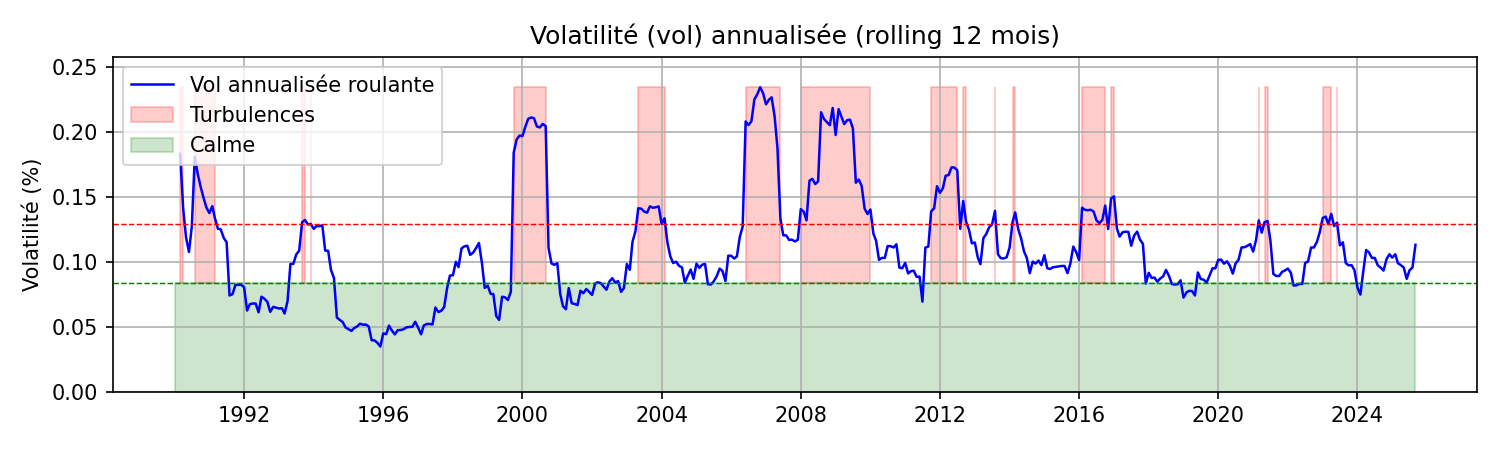
\includegraphics[width = 0.9\textwidth]{gold_volatility_zones.png}
    \caption{Illustration de la volatilité sur le cours de l'or}
    \label{fig:gold_volatility_zones}
\end{figure}



%%%%%%%%%%%%%%%%%%%%%%%%%%%%%%%%%%%%%%%%%%%%%%%%%%%%%%%%%%%%%%%%%%%%%%%%%%%%%
%%%%%%%%%%%%%%%%%%%%%%%%%%%%%%%%%%%%%%%%%%%%%%%%%%%%%%%%%%%%%%%%%%%%%%%%%%%%%
%%%%%%%%%%%%%%%%%%%%%%%%%%%%%%%%%%%%%%%%%%%%%%%%%%%%%%%%%%%%%%%%%%%%%%%%%%%%%
\section{ADF~: Augmented Dickey–Fuller - Tests de stationnarité}

Le test ADF (Augmented Dickey--Fuller) sert à déterminer si une série
temporelle est stationnaire ou non. L'hypothèse nulle est que la
série a une racine unitaire (non-stationnarité), et l'hypothèse
alternative est que la série est stationnaire.

On l'applique sur $\ln(P_t)$ (niveau) et sur les rendements
logarithmiques. En pratique~:
\begin{itemize}
  \item les niveaux $\ln(P_t)$ sont souvent non-stationnaires,
        car les prix s'accumulent avec le temps et présentent une
        tendance~;
  \item les rendements logarithmiques $RLog$ sont souvent
        stationnaires, fluctuant autour d'une moyenne stable avec
 une variance relativement constante.
\end{itemize}

\paragraph{Intuition physique / signal}

Une série non-stationnaire peut être vue comme un signal cumulé,
semblable à une marche aléatoire. Les rendements log sont la "dérivée"
de ce signal, plus proche d'un bruit stationnaire. Le test ADF
indique donc si l'on peut traiter une série comme stable ou s'il
faut la différencier pour éliminer la tendance.

%%%%%%%%%%%%%%%%%%%%%%%%%%%%%%%%%%%%%%%%%%%%%%%%%%%%%%%%%%%%%%%%%%%%%%%%%%%%%
%%%%%%%%%%%%%%%%%%%%%%%%%%%%%%%%%%%%%%%%%%%%%%%%%%%%%%%%%%%%%%%%%%%%%%%%%%%%%
%%%%%%%%%%%%%%%%%%%%%%%%%%%%%%%%%%%%%%%%%%%%%%%%%%%%%%%%%%%%%%%%%%%%%%%%%%%%%
\section{Indicateurs de performance globale}

%%%%%%%%%%%%%%%%%%%%%%%%%%%%%%%%%%%%%%%%%%%%%%%%%%%%%%%%%%%%%%%%%%%%%%%%%%%%%
\subsection{CAGR~: Compound Annual Growth Rate}

Le taux de croissance annuel composé (CAGR) mesure le rendement géométrique moyen 
d'un actif sur une période donnée. Il est défini par~:
\begin{equation}
    CAGR = \left(\frac{P_T}{P_0}\right)^{1/n_{ann}} - 1,
\end{equation}
où $P_0$ est le prix initial, $P_T$ le prix final et $n_{ann}$ le nombre d'années.

Le CAGR est utile car il résume la performance d'un actif en un seul taux annuel 
équivalent, prenant en compte la capitalisation composée, contrairement au rendement 
arithmétique moyen qui ignore l'effet de la composition.

\paragraph{Exemples de croissance~:} 

Pour doubler le capital en $n$ années, on résout
\[
2 = (1 + CAGR)^n \quad \Rightarrow \quad CAGR = 2^{1/n} - 1.
\]

\begin{itemize}
    \item Pour doubler en 5 ans~: 
    \[
    CAGR = 2^{1/5} - 1 \approx 0.149 \; \Rightarrow 14.9\% \text{ annuel}
    \]
    \item Pour doubler en 10 ans~: 
    \[
    CAGR = 2^{1/10} - 1 \approx 0.072 \; \Rightarrow 7.2\% \text{ annuel}
    \]
\end{itemize}

Ainsi, un actif avec un CAGR d'environ 7\% par an double approximativement sur 10 ans, 
et un actif avec 15\% par an double sur 5 ans. Cela permet de relier directement 
le CAGR à des objectifs de croissance concrets.



%%%%%%%%%%%%%%%%%%%%%%%%%%%%%%%%%%%%%%%%%%%%%%%%%%%%%%%%%%%%%%%%%%%%%%%%%%%%%
\subsection{Volatilité historique}

La volatilité historique mesure l'amplitude des variations du prix de
l'or au fil du temps. Elle est calculée sur l'ensemble des rendements
logarithmiques, puis annualisée pour être comparable aux autres actifs~:
\begin{equation}
    \sigma_{hist} = \sqrt{12} \; \mathrm{std}(RLog).
\end{equation}

\paragraph{Interprétation~:} 

- $\sigma_{hist}$ exprime la dispersion du rendement annuel moyen.  
- Par exemple, une volatilité de 12~\% signifie qu'environ 68~\%
  (1 écart-type autour de la moyenne de la gaussienne)
  des rendements annuels observés se situent dans $\pm 12\%$ autour de
  la moyenne.  
- Pour l'or, historiquement, la volatilité annuelle typique se situe
  entre 10~\% et 20~\% selon les périodes de marché.  
- Une volatilité élevée indique un marché agité et plus risqué, tandis
  qu'une faible volatilité correspond à un marché calme.  
- Comparée à des actions (volatilité typique de 20-30~\%) ou à des
  obligations (3-10~\%), l'or présente souvent une volatilité
  intermédiaire, mais avec des pics en période de crise financière.


\begin{table}[h!]
\centering
\begin{tabular}{lccc}
\toprule
Période & Évènement &S\&P 500 (\%) & Or (\%) \\
\midrule
1929--1932  & Grande Dépression             & 50--60  & 10--15 \\
1973--1974  & choc pétrolier                & 35--40  & 20--25 \\
1987        & krach "lundi noir"            & 25--30  & 15--20 \\
2000--2002  & bulle tech                    & 20--25  & 10--15 \\
2007--2009  & crise financière              & 25--30  & 25--30 \\
2020        & Covid                         & 30--35  & 20--25 \\
2022        & inflation / guerre Ukraine    & 25--30  & 15--20 \\
\bottomrule
\end{tabular}
\caption{Volatilité approximative annuelle en période de crise pour S\&P 500 et l'or (USD)}
\label{tab:volatility_crises}
\end{table}


%%%%%%%%%%%%%%%%%%%%%%%%%%%%%%%%%%%%%%%%%%%%%%%%%%%%%%%%%%%%%%%%%%%%%%%%%%%%%
\subsection{Max Drawdown - Perte maximale}

Le \emph{maximum drawdown} (MDD) représente la perte maximale qu'un 
investisseur aurait subie s'il avait acheté au sommet historique et vendu
au point le plus bas suivant. Mathématiquement~:
\begin{equation}
    MDD = \min_t \left(\frac{P_t}{\max_{s\le t} P_s} - 1\right),
\end{equation}
où $P_t$ est le prix de l'actif à l'instant $t$.

Cette mesure capture le risque extrême et est utilisée pour évaluer la
robustesse d'un portefeuille face aux baisses sévères. Contrairement à la
volatilité, le MDD se concentre uniquement sur les pertes et non sur la
variabilité totale des rendements.

\begin{table}[h!]
\centering
\begin{tabular}{lccc}
\toprule
Période & Évènement & S\&P 500 (\%) & Or (\%) \\
\midrule
1929--1932  & Grande Dépression             & 80--86  & 0--10 \\
1973--1974  & Choc pétrolier                & 45--48  & -5--0 \\
1987        & Krach "lundi noir"            & 30--33  & -5--0 \\
2000--2002  & Bulle tech                    & 45--49  & 5--10 \\
2007--2009  & Crise financière              & 55--57  & 20--25 \\
2020        & Covid                         & 30--34  & 0--5 \\
2022        & Inflation / guerre Ukraine    & 20--25  & -5--0 \\
\bottomrule
\end{tabular}
\caption{Max drawdown (perte maximale) historique approximatif pour le S\&P 500 et
l'or (USD) lors des crises majeures. Les valeurs négatives montrent que l'or
-- sur la période -- s'est valorisé.}
\label{tab:mdd_crises}
\end{table}

\noindent
On remarque que les actions peuvent perdre plus de la moitié de leur valeur
lors de crises majeures, alors que l'or a souvent joué un rôle de valeur
refuge, limitant ses pertes ou générant des gains même en période de
turbulences.




\end{document}
